\documentclass[10pt, a4paper]{report}


\usepackage[left=15mm, top=20mm, right=15mm, bottom=20mm]{geometry}

\usepackage[utf8]{inputenc}
\usepackage[english,russian]{babel}
\usepackage{mflogo}
\usepackage{amsmath,amsfonts,amssymb}
\usepackage{xcolor}
\usepackage{graphicx}
\usepackage{cite}
\usepackage{multicol}
\usepackage{url}

\usepackage{titlesec}
\usepackage{theoremref}
\usepackage{setspace}
\usepackage{amsthm,amsmath}
\usepackage[shortlabels]{enumitem}

\renewcommand{\qedsymbol}{$\blacksquare$}

\newtheorem{theorem}{Теорема}[chapter]
\newtheorem{lemma}{Лемма}
\theoremstyle{definition}
\newtheorem{remark}{Предложение}[chapter]

\renewcommand{\Im}{\mathop{\mathrm{Im}}\nolimits}
\renewcommand{\Re}{\mathop{\mathrm{Re}}\nolimits}
\renewcommand{\cot}{\mathop{\mathrm{ctg}}\nolimits}
\renewcommand{\sinh}{\mathop{\mathrm{sh}}\nolimits}
\renewcommand{\cosh}{\mathop{\mathrm{ch}}\nolimits}
\renewcommand{\arctan}{\mathop{\mathrm{arctg}}\nolimits}
\renewcommand{\tan}{\mathop{\mathrm{tg}}\nolimits}
\renewcommand{\tanh}{\mathop{\mathrm{th}}\nolimits}
\renewcommand{\sinh}{\mathop{\mathrm{sh}}\nolimits}
\renewcommand{\cosh}{\mathop{\mathrm{ch}}\nolimits}
\renewcommand{\coth}{\mathop{\mathrm{ctgh}}\nolimits}
\renewcommand{\log}{\ln}
\DeclareMathOperator{\lcm}{lcm}


\titleformat{\chapter}{\Large\bfseries}{}{0pt}{\huge} 

\setlength{\parskip}{0.5cm}

\graphicspath{{images/}}

\title{Оценка числа компонент графа итерации случайного отображения}
\author{Автор: Михалицын Пётр Константинович \\ Научный руководитель: Старший преподаватель кафедры "Компьютерная безопасность" \\ Миронкин Владимир Олегович}
\date{30 апреля 2018 г.}

\begin{document}
\thispagestyle{empty}
\large
\begin{singlespacing}
	\begin{center}
		
		ПРАВИТЕЛЬСТВО РОССИЙСКОЙ ФЕДЕРАЦИИ\\
		\vspace{0.5cm}
		Федеральное государственное автономное образовательное\\
		учреждение высшего профессионального образования\\
		Национальный исследовательский университет\\
		<<Высшая школа экономики>>\\
		\vspace{0.5cm}
		Московский институт электроники и математики им.\,А.Н.\,Тихонова \\
		Департамент прикладной математики\\
		Кафедра <<Компьютерная безопасность>>
		
		\vspace{2.5cm}
		
		
		{\bf КУРСОВАЯ РАБОТА}\\
		по дисциплине <<Теория информации>>\\[2ex]
		<<Оценка числа компонент графа итерации случайного отображения>>
		
		
		\vspace{5cm}
		
		
		\begin{tabular}{ll}
			\hspace{9cm} & \underline{Выполнил:}\\
			& студент группы СКБ-151\\
			& Михалицын П.К.\\
			& \underline{Проверил:}\\
			&  старший преподаватель кафедры\\
			& <<Компьютерная безопасность>>\\
			&  Миронкин~В.О.
		\end{tabular}
		
	\end{center}
	\vfill
	\begin{center}
		МОСКВА 2018
	\end{center}
\end{singlespacing}
\normalsize

\tableofcontents

\chapter*{Введение}
\addcontentsline{toc}{chapter}{Введение}
В данной работе мы выведем формулы среднего числа компонент, получаемых при итерации случайного отображения. Отдельно будут рассмотрены случаи биективного отображения и оценка среднего максимального числа компонент при итерации. В вводной части, будет рассмотрен случай, когда итерации не производятся -- для лучшего освоения материала и вывода основных вспомогательных формул, которые мы рассмотрим в уже основной части данной работы. 

Эта работа будет полезна в алгоритмах шифрования и выработки ключа, особенно в получении оценки максимального количества итераций, при которых можно использовать данный ключ при взятии случайного отображения, для уменьшения вероятности вхождения в цикл. Таким образом можно оценивать количество непересекающихся множеств ключей, которые будут создавать те самые компоненты графа. 

Существует возможность расширения области применения данной работы до приложений в сферах, которые были указаны выше. Всего этого можно добиться, без труда выведя небольшое количество формул. т.к. основные формулы и концепции их получения будут рассмотрены в данной работе.

\chapter{Оценка числа компонент графа отображения}

\section{Случай любого случайного отображения}
Прежде чем начать поиск числа компонент графа случайного отображения, определим как выглядит граф этого отображения.

В первую очередь рассмотрим пример графа случайного отображения, чтобы понять с чем мы будем иметь дело и что считать.

\begin{figure}[h]
	\centering
	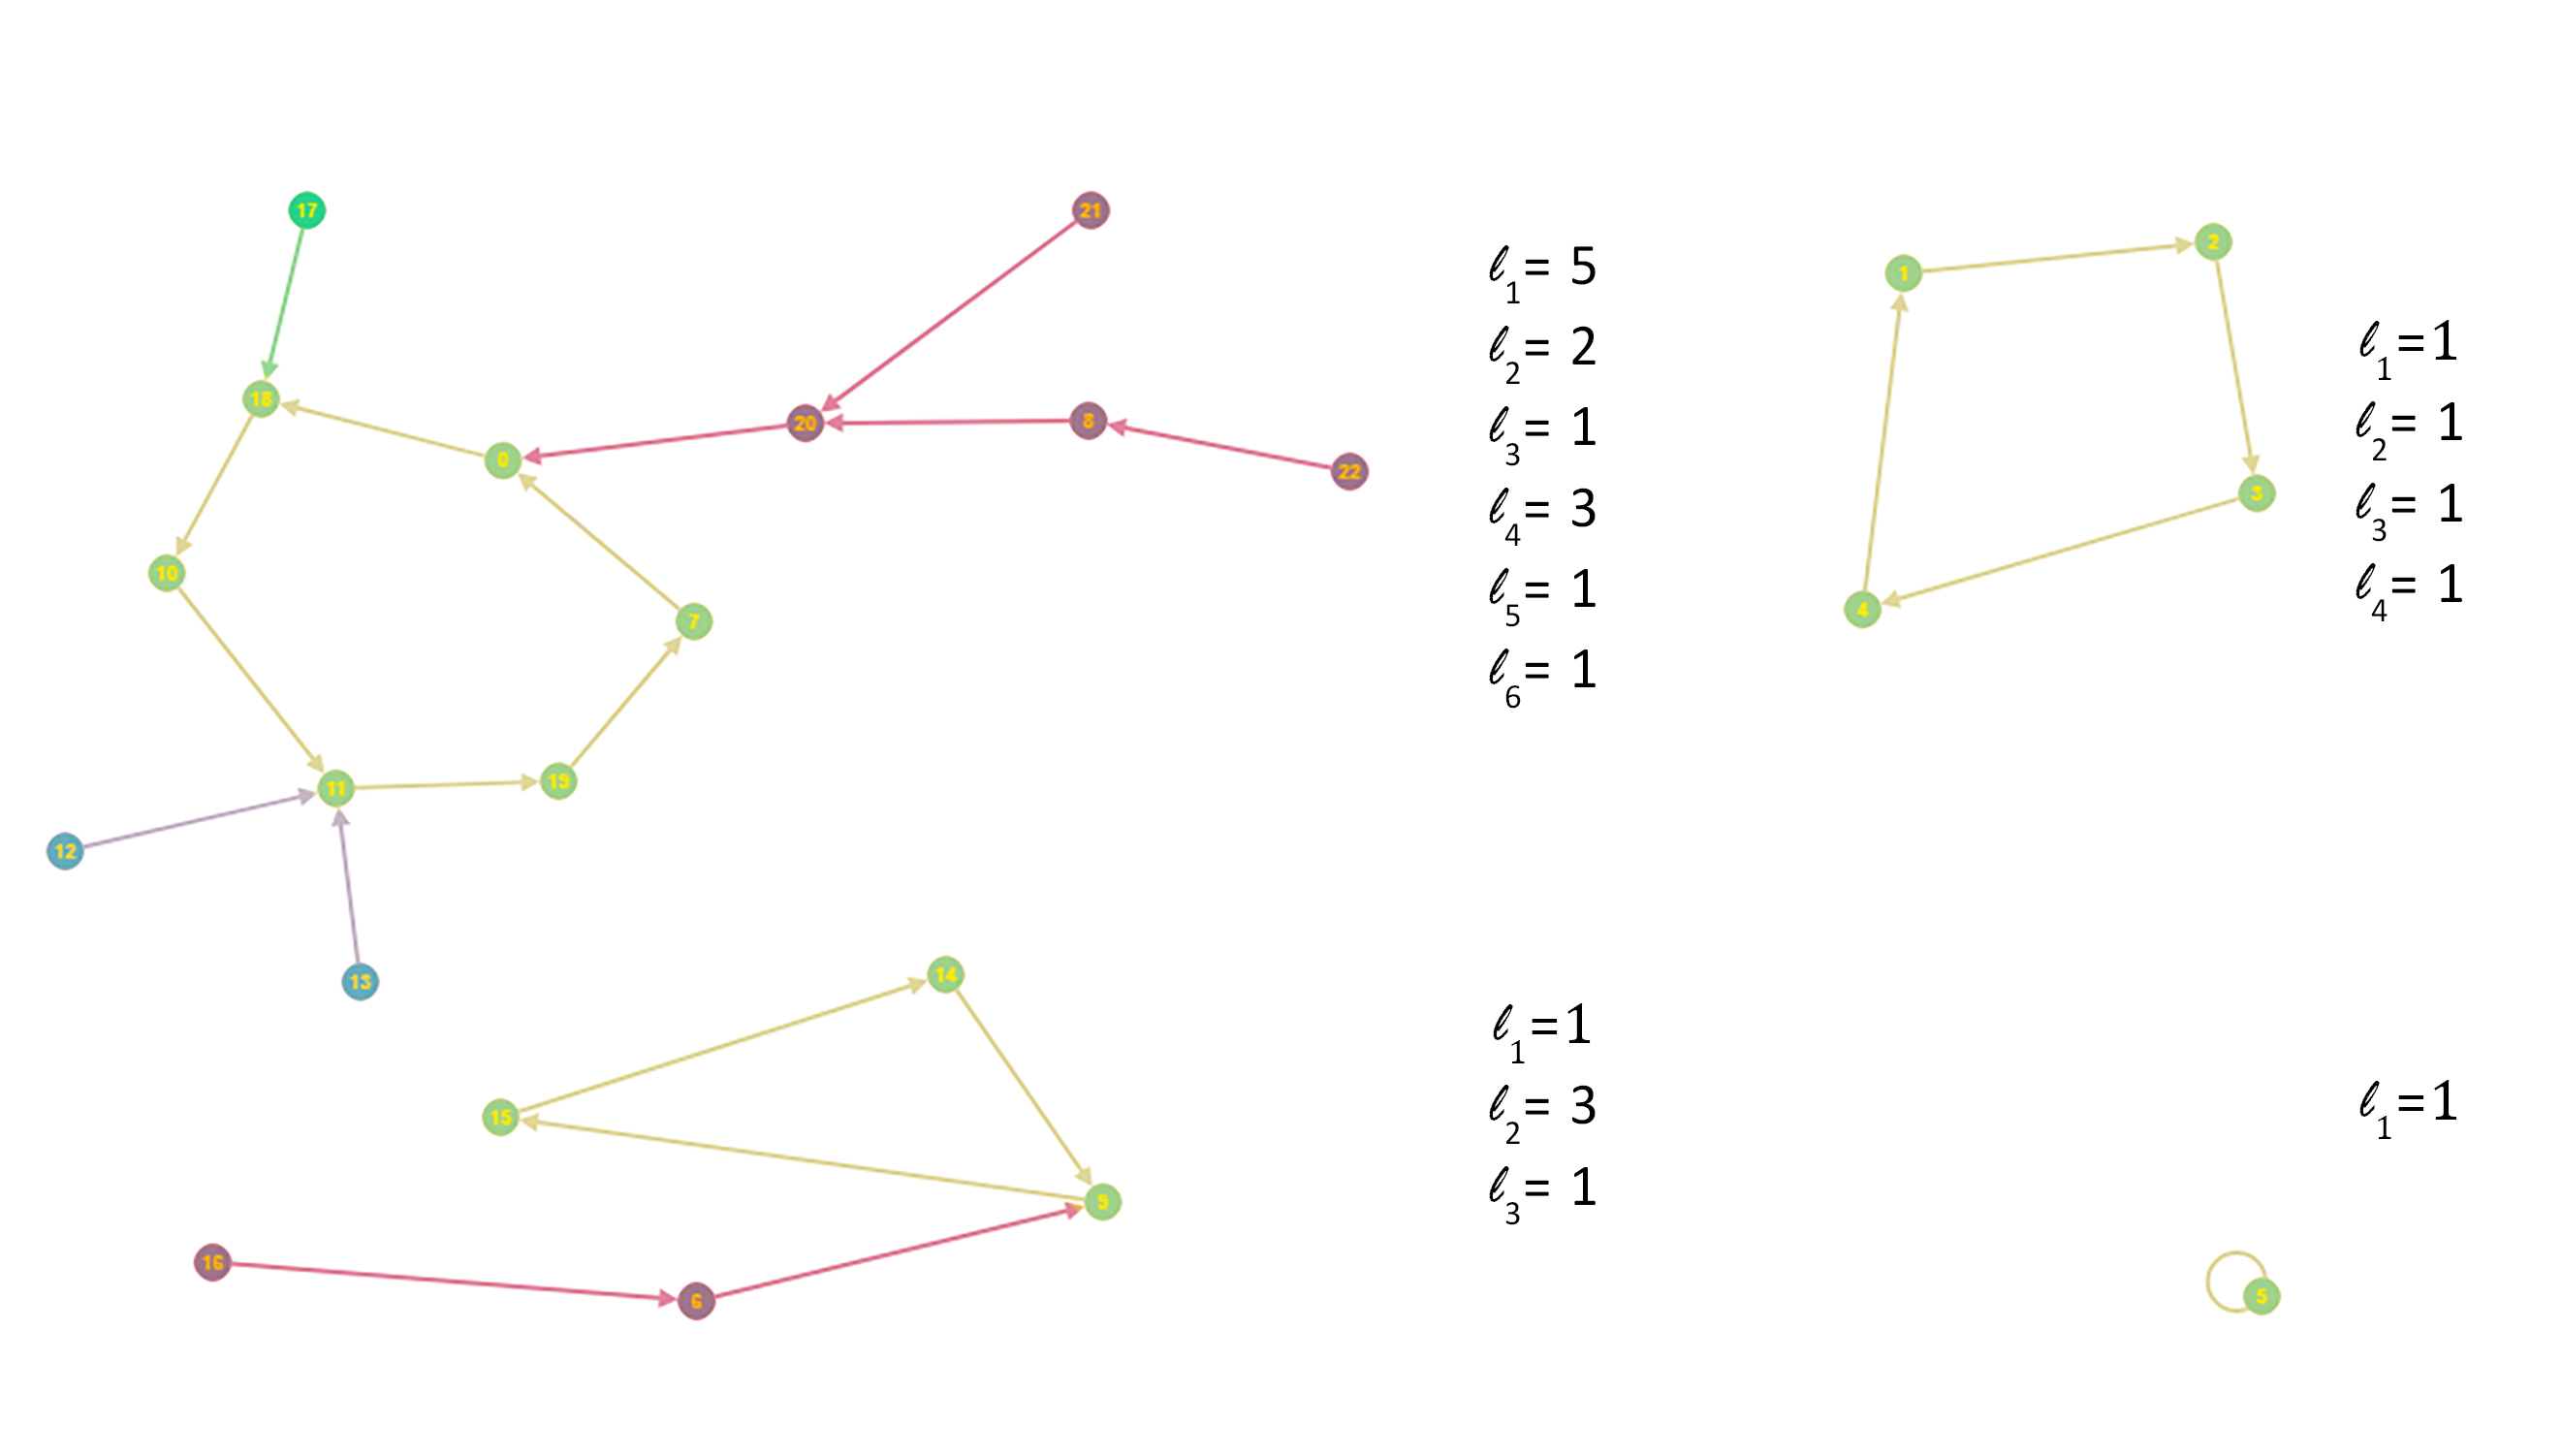
\includegraphics[width=0.75\textwidth]{graph_ex.jpg}
	\caption{Пример графа случайного отображения}
	\label{graph_ex}
\end{figure}

Очевидно, что будет образовываться некоторое подобие леса. Причем каждая компонента этого леса будет ориентированным графом ровно с одним циклом, более того все ребра будут направлены в сторону этого цикла.

Теперь давайте приступим к подсчету количества таких графов. Для начала начнем с одной компоненты. Введем следующие параметры, которые могут определить данную компоненту и определим число компонент с данными параметрами.

\begin{enumerate}
\item $n$ -- кол-во вершин в компоненте
\item $l_1, l_2, ..., l_k$ -- число вершин, находящихся в "побочных путях"{}, ведущих до циклической части графа, (каждая из них больше $0$ и при этом в сумме они дают $n$). Стоит заметить, что под побочными путями имеются в виду ориентированные деревья, каждая из вершин которых имеет однозначный путь до цикла (в силу того, что это деревья)
\item $k$ -- число вершин в цикле
\end{enumerate}
Для наглядности на рисунке \ref{graph_ex} желтым цветом определен цикл, а другими цветами определены побочные компоненты и указаны соответствующие параметры графа.


Приступим к подсчетам.

Для первого "побочного пути"{} нужно выбрать какие вершины  будут в нем состоять ($\frac{n!}{l_1!(n - l_1)!}$ способов) После этого нужно будет разместить их на дереве, которое будет соединено впоследствии с циклом. Согласно теореме Келли о числе деревьев : $l_1^{l_1-2}$ -- количество различных деревьев, которые можно построить на $l_1$ вершинах. После этого на собранном дереве нужно будет выбрать вершину, которая окажется в цикле ($l_1$ способов). Очевидно, что выбирая на дереве вершину, которая будет в цикле мы всегда однозначным образом определяем направление, в котором будут идти стрелки от каждой другой вершины до выбранной(т.к. в дереве, кратчайший путь от одной вершины к другой всегда однозначен и в нем отсутствуют циклы). Итого получим кол-во способов выбора такого "побочного пути":
$$\frac{n!}{l_1!(n- l_1)!} l_1^{l_1-1}$$


Проделав то же самое для второго побочного пути, получим кол-во возможных комбинаций:
$$\frac{(n- l_1)!}{l_2!(n- l_1 - l_2)!} l_2^{l_2-1}$$


 и т.д. для $k$ой компоненты получим кол-во способов:
$$
\frac{(n - l_1 - ... -l_{k-1})!}{l_k!(n - l_1 - l_2 - ... - l_k)!} l_k^{l_k-1}=
\frac{(n - l_1 - ... -l_{k-1})!}{l_k!}l_k^{l_k-1}
$$

Осталось определить как будут расположены вершины на цикле ($(k-1)!$ способов. Мы убрали оттуда $k$ т.к. любую из этих вершин можно считать начальной)

Перемножая полученные комбинаторные значения, получаем итоговую формулу:

$$
(k-1)!\frac{n!}{l_1!(n - l_1)!} l_1^{l_1-1} * ... * \frac{(n - l_1 - ... -l_{k-1})!}{l_k!} l_k^{l_k-1}=
(k-1)!C^{l_1, l_2, ..., l_k}_n l_1^{l_1-1}l_2^{l_2-1}...l_k^{l_k-1}
$$
, где $C^{l_1, l_2, ..., l_k}_n$ -- мультиномиальный коэффициент,

Теперь нужно просуммировать данные значения при различных $l_1, l_2, ..., l_k$ и учитывая возможное возникновение повторений при подсчете, получим итоговую формулу для подсчета количества числа таких компонент.

$$
\sum_{k=1}^{n}\frac 1 {k}\sum_{l_1+l_2+...+l_k=n} C^{l_1, l_2, ..., l_k}_n l_1^{l_1-1}l_2^{l_2-1}...l_k^{l_k-1}=
$$
Полученные числа, показывают кол-во определенных выше компонент графа (один цикл и все побочные компоненты ведут к нему), которые можно построить на $n$ вершинах. Обозначим их $M(n)$.


Стоит заметить, что данные числа встречаются в работе Дональда Кнута "Искусство программирования". В онлайн энциклопедию целочисленных последовательностей они занесены под номером A001865 и обозначают количество функций, у которых соответствующий им граф отображения имеет одну компоненту связанности (Number of connected functions on n labeled nodes)\cite{Main-lib}.

В этой же энциклопедии имеется более простая формула для вычисления этих последовательностей, а именно имеет место теорема, которую мы оставим без доказательства

\begin{theorem}
Суммарное число компонент графов случайных эндоморфизмов над алфавитом мощности $n$ можно подсчитать по формуле

\begin{equation}
	\label{M-coef}
	\sum_{k=1}^n \frac{n!n^{n-k-1}}{(n-k!)}
\end{equation}

Причем $k$ое слагаемое внутри суммы -- это количество искомых графов, в которых содержится цикл длины $k$.
\end{theorem}

Зная данный факт, давайте попробуем найти экспоненциальную производящую функцию для данных чисел, т.к. после этого вычисление данных чисел будет занимать всего одну строчку кода в пакете Wolfram Mathematica и к тому же этот подсчет будет происходить гораздо быстрее. 

\begin{theorem}
	Экспоненциальной производящей функцией для количества отображений, которые имеют одну компоненту связанности, является 

$$-\ln(1+W(-x))$$
, где $W(x)$ --W функции Ламберта\cite{W-lib}

\end{theorem}

\begin{proof}

$$
W(x) = \sum_{n=0}^{\infty} (-1)^{n-1}\frac{n^{n-1}x^n}{n!}
$$ 

Зная замечательное свойство ряда Тейлора для степени W-функции Ламберта:

$$
W^k(x) = -k \sum_{n=k}^\infty \frac{(-n)^{n-k-1}}{(n-k)!}x^n
$$ 
увидим, что данная формула очень напоминает слагаемые той, которую мы нашли в онлайн энциклопедии для наших чисел. А именно, если мы рассмотрим такую функцию:

\begin{equation}
\label{cycle-coef}
(-1)^{k} \frac{W^k(-x)}{k} =  \sum_{n=k}^\infty \frac{n^{n-k-1}}{(n-k)!}x^n
\end{equation} , то заметим, что именно она будет являться экспоненциальной производящей функцией для количества односвязанных искомых графов с циклом длины $k$

Теперь, если мы рассмотрим ряд Тейлора от функции:

$$
- W(-x) + \frac{W^2(-x)}{2} - \frac{W^3(-x)}{3} + \frac{W^4(-x)}{4} - ... =
$$ , то коэффициент при $x^n$ будет в точности как из формулы \eqref{M-coef}. Обнаружим, что такой ряд имеет именно функция 

$$
-\log(1+W(-x))
$$
\end{proof}

Осталось только определить число графов, состоящих из таких компонент, построенных на $n$ вершинах. 
Если в каждой компоненте будет $n_i$ вершин, а всего компонент $k$, то искомое число таких графов

\begin{equation}
\label{useless-coef}
\frac 1 {k!} \sum_{n_1+n_2+...+n_k=n} C^{n_1, n_2, ..., n_k}_n M(n_1)M(n_2)...M(n_k)
\end{equation}

\begin{remark}
	Экспоненциальная производящая функция для этих чисел будет
	
	\begin{equation}
	\label{W-coef}
	(-1)^k \frac 1 {k!} \ln^k(1+W(-x))
	\end{equation}
	
	Действительно, если мы будем возводить наш ряд в степень $k$, то перед $x^n$ будет находиться число, стоящее в формуле в соответствии со свойствами возведения в степень экспоненциальных производящих функций
\end{remark}


Данная особенность получения чисел с помощью экспоненциальной производящей функции позволит нам упростить расчеты, сделать их более эффективными в плане вычислений. Так на компьютере автора поиск искомых чисел с помощью формулы \eqref{useless-coef} позволял работать только с алфавитом мощности 20-30, в то время как работа с помощью формулы \eqref{W-coef} позволила добиться увеличения производительности в десятки раз. В анализе полученных результатов мы получим явные формулы для данных чисел, которые повысят производительность вычислений уже в сотни раз.

Теперь приступим к подсчету чисел, ради которых и была написана данная глава этой работы--подсчету суммарного числа компонент всех графов отображений. Зная суммарное число компонент можно без особых трудностей получить среднее поделив суммарное число компонент на количество всех функций ($n^n$).

\begin{theorem}
	Суммарное число компонент графов всех эндоморфизмов можно получить с помощью экспоненциальной производящей функции
	$$\frac{-\log(1+W(-x))}{(1+W(-x))}$$
\end{theorem}

\begin{proof}
Поскольку мы знаем, как получить число наших графов с $n$ вершинами обладающими $k$ компонентами (воспользовавшись тем фактом, что это $n$ый коэффициент в ряду Тейлора у функции \eqref{W-coef}), попробуем узнать вид экспоненциальной производящей функции, коэффициенты ряда Тейлора которого -- суммарное число компонент всех графов соответствующие всем эндоморфизмам над множеством мощности n.

Если мы знаем кол-во графов с одной компонентой, двумя, тремя и т.д., то суммарное число компонент, это сумма произведений числа графов с k компонентами умноженными на k, где $k=1,...,n$.

т.к. эти числа лежат в коэффициентах функций вида \eqref{W-coef}, то проделаем несколько манипуляций с этими функциями:

$$\sum_{k=1}^{n} k (-1)^k \frac 1 {k!} \ln^k(1+W(-x))= 
\sum_{k=1}^{n} \frac 1 {(k-1)!} (-\ln(1+W(-x)))^k
$$

Заметим, что свободный коэффициент в \eqref{W-coef} всегда равен 0 (число отображений в графе с $n=0$ вершинами на $k\ne0$ компонентами равно 0). Поэтому с увеличением мощности алфавита и при произведении расчетов для эндоморфизмов над алфавитом мощности $n$, первые $k<n$ компонент будут такими же как и для эндоморфизмов над алфавитом мощности $k$ т.к. в нашей формуле появится только $-\ln(1+W(-x))$ в степени $n$, а значит первые $k<n$ коэффициентов не изменятся.

Таким образом мы можем сделать переход до $n=\inf$ и взять оттуда нужные нам коэффициенты.  

$$
\sum_{k=1}^{\infty} \frac 1 {(k-1)!} p^k=
e^p*p
$$

Делая обратно подстановку $p=-\ln(1+W(-x))$ Получим:

$$
\frac {-\ln(1+W(-x))}{(1+W(-x))}
$$
\end{proof}

\begin{remark}
	Для того, чтобы узнать среднее количество компонент графов функций над алфавитом мощности $n$ нужно взять $n$ый член ряда Тейлора полученной функции и поделить его на общее число функций ($n^n$). Как уже отмечалось выше, сам $n$ый коэффициент означает суммарное число компонент графа от всех отображений над алфавитом мощности $n$.
\end{remark}

\section{Случай биективного случайного отображения}

Формула, полученная выше, решает задачу для случая любой функции (не обязательно биективной). В связи с тем, что автор находит весьма красивым формулу для суммарного числа компонент графов биективных отображений, мы рассмотрим этот случай отдельно от функций общего вида.

В первую очередь заметим, что если мы будем рассматривать случай биективной функции, то графы, которые будут образовываться представят собой циклы.

Выведем формулу для подсчета кол-ва способов разбиения множества k на различные непересекающиеся циклы. Данная задача уже будет выглядеть довольно простой в сравнении с предыдущей задачей, связанной с любой функцией. 

Рассмотрим случай, когда мы разбили наше множество на $k$ циклов длины $l_1, l_2, ..., l_k$. 

\begin{remark}
Можно заметить что данные числа являются числами Стирлинга первого рода без знака и для них существует простая рекуррентная формула для подсчета.
\end{remark}

Эта "особенность" не является случайной. Если внимательно посмотреть на определение чисел Стирлинга первого рода, то можно понять, что это именно те числа, которые мы и хотели получить изначально. А именно это количество перестановок из n элементов с k циклами.

\begin{theorem}
Для вычисления чисел Стирлинга первого рода существует рекуррентное соотношение 

$$S(n, k) = S(n-1, k-1) + (n-1) S(n-1,k)$$
$$S(0,0) = 1$$
$$S(n,0) = 0, \text{ при } n>0$$
$$S(0,k) = 0, \text{ при } k>0$$
\end{theorem}
\begin{proof}
Смысл этого рекуррентного соотношения следующий. Для разбиения множества из $n$ элементов на $k$ циклов, можно взять уже готовое разбиение множества с $n-1$ элементами на $k-1$ циклов и добавить новый элемент в качестве нового цикл или же можно было взять разбиение множества c $n-1$ элементами на $k$ циклов и добавить новый элемент в один из готовых циклов ($n-1$ способ). 
\end{proof}

Теперь приступим к подсчету среднего количества компонент графа. Обозначим через $A(n)$ это количество для языка мощности $n$ при биективном отображении

$$A(n) = \frac 1 {n!}(1*S(n,1)+2*S(n,2)+...+n*S(n,n))=$$
$$\frac 1 {n!} (1*(S(n-1,1-1)+(n-1)*S(n-1,1))+2*((S(n-1,2-1)+(n-1)*S(n-1,2)))+...+n*((S(n-1,n-1)+(n-1)*S(n-1,n))))=$$
$$\frac 1 {n!} (1*((n-1)*S(n-1,1))+2*((S(n-1,2-1)+(n-1)*S(n-1,2)))+...+n*((S(n-1,n-1))))=$$
$$\frac 1 {n!} ((n-1)*(1*S(n-1,1)+2*S(n-1,2)+...+(n-1)*S(n-1,n-1)) + 2*S(n-1,1)+3*S(n-1,2)+...+n*S(n-1,n-1))=$$
$$\frac 1 {n!} (n*(1*S(n-1,1)+2*S(n-1,2)+...+(n-1)*S(n-1,n-1)) + S(n-1,1)+S(n-1,2)+...+S(n-1,n-1))=$$
$$\frac 1 {n!} (n*A(n-1) + (n-1)!)=$$

Очевидно, что $A(1)=1$.
Теперь от рекурсивной функции перейдем к непосредственной 

$$A(n) = \frac 1 {n!} (n*A(n-1) + (n-1)!) = \frac 1 {n!} (n*((n-1)A(n-2)+(n-2)!) + (n-1)!)=$$
$$\frac 1 {n!} (n*((n-1)((n-2)A(n-3)+(n-3)!)+(n-2)!) + (n-1)!)=$$
$$\frac 1 {n!} (n*((n-1)((n-2)A(n-3)+(n-3)!)+(n-2)!) + (n-1)!)=$$
$$\frac 1 {n!} (n*((n-1)((n-2)(...3(2*1+1!)+2!)...+(n-3)!)+(n-2)!) + (n-1)!)=$$
$$\frac 1 {n!} (n!+\frac{n!}{2}+\frac{n!}{3}+...+\frac{n!}{n-1}+\frac{n!}{n})=$$
$$ 1+\frac{1}{2}+\frac{1}{3}+...+\frac{1}{n-1}+\frac{1}{n}= \sum_{k=1}^n \frac 1 k$$

\begin{theorem}
Среднее количество компонент графа, относящееся к биективному отображению над алфавитом мощности $n$ на себя, является $n$ым гармоническим числом.
\end{theorem}

\begin{remark}
Этот факт показывает например, что с увеличением мощности алфавита число компонент стремится к бесконечности (из свойств гармонических чисел).
\end{remark}

\section{Анализ полученных формул}

Для того, чтобы начать анализ полученных формул давайте найдем непосредственно формулу для количества компонент графа случайного отображения. Для этого рассмотрим экспоненциальную функцию, которую мы получили.

$$
\frac{-\log (1+W(-x))}{1+W(-x)}
$$

посмотрим, какой коэффициент будет при $x^n/n!$

$$
\frac{-\log (1+W(-x))}{1+W(-x)} = (- W(-x) + \frac{W^2(-x)}{2} - \frac{W^3(-x)}{3} + \frac{W^4(-x)}{4} - ...) (1 -W(-x) + W^2(-x) - W^3(-x) + W^4(-x) - ...)=
$$
$$
\sum_{k=1}^{\infty}H(k)(-W(-x))^k
$$, где $H(n)$ -- $n$ое гармоническое число.

Т.к. мы знаем краткую формулу ряда Тейлора для $(-W(-x))^k$

$$
\sum_{k=1}^{\infty}H(k)\sum_{n=k}^{\infty} \frac{k n^{n-k-1} n!}{(n-k)!} \frac{x^n}{n!}
$$ 

и коэффициент при $x^n$ появляется только если $k=1,...,n$, то получим итоговую формулу для коэффициента при $x^n/n!$

$$
\sum_{k=1}^{n}H(k) \frac{k n^{n-k-1} n!}{(n-k)!}
$$

Отсюда получаем
\begin{theorem}
Среднее число компонент в графе случайного отображения будет задаваться формулой

$$
\sum_{k=1}^{n}H(k) \frac{k n^{-k-1} n!}{(n-k)!}
$$
\end{theorem}
Данная формула еще больше повышает производительность вычислений. 

\begin{remark}

В вышеуказанной онлайн энциклопедии имеется формула, показывающая к какой функции асимптотически сходится данная сумма \cite{Asympt-lib}, а именно

$$
\frac{(\log(2n)+\gamma)}2
$$, где $\gamma$ -- константа Эйлера
\end{remark}
Данный результат хорошо приближает вычисления. Так, например, на графике ниже представлена зависимость значения среднего числа компонент от мощности языка, 

\begin{figure}[h]
	\centering
	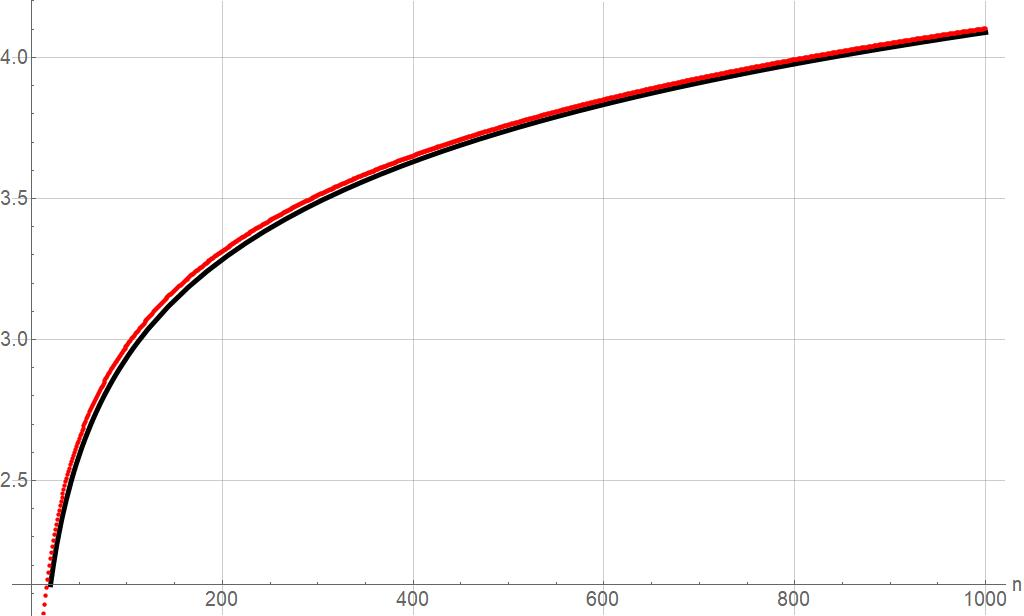
\includegraphics[width=0.75\textwidth]{Comp1.jpg}
	\caption{График зависимости среднего числа компонент графа отображения от мощности языка}
	\label{comp1}
\end{figure}

Как видно из этого графика, данная функция действительно хорошо приближает значение среднего числа компонент, так для мощности языка $10000$ погрешность в вычислениях меньше $10^{-2}$

Про асимптотику числа компонент нет смысла говорить в связи с тем, что гармонический ряд аппроксимируется  данной функцией:
$$
\log{n}+\gamma
$$ и это является общеизвестным фактом.

\chapter{Оценка числа компонент графа итерации случайного отображения}

\section{Основная часть}

Перейдем теперь к сути исходной задачи, которая стояла  перед нами, а именно как будет изменяться суммарное число компонент графа при итерации случайного отображения.

В первую очередь заметим, что при итерации отображения мы будем перепрыгивать через несколько ребер нашего графа, причем в результате данных "прыжков" циклы могут распадаться и собираться вместе. Из этого свойства следует один из важных фактов, который позволит вычислить при какой степени суммарное число компонент графа будет максимальным. Давайте рассмотрим при каком условии наши компоненты содержащие циклы различной длины распадутся на компоненты с циклами длиной 1. Такое возможно если в цикле любой длины мы будем возвращаться обратно в свою же вершину. Для этого нужно, чтобы степень отображения делилась на длину любого цикла в компонентах, то есть была наименьшим общим кратным для всех чисел, начиная с единицы и заканчивая длиной самого максимального цикла (то есть мощности алфавита). То есть, например, для 5 это число будет $\lcm(1,2,3,4,5) = 60$.
 
Запишем этот факт в качестве предложения
\begin{remark}
	Суммарное чило образовавшихся компонент графа в результате итерации случайного отображения над алфавитом мощности $n$ максимально в том случае, когда итерация происходит $i\lcm(1,2,...,n)$, где $i=1,2,...$ 
\end{remark}

Данный факт мы оставим на рассмотрение в следующем разделе, а теперь перейдем к основной задаче. Начнем с нахождения количества компонент,на которые распадется одна компонента графа при возведении случайного отображения в степень $r$. Имеет место теорема
\begin{theorem}\thlabel{thrm:compcount}
	 Если компонента с циклом длины $k$, то число компонент, на которое распадется данная компонента при возведении отображения в степень $r$ будет $\gcd(r,k)$.
\end{theorem}

\begin{proof}
	
	Пусть $n$ -- минимальное число вершин, которые мы пройдем до попадания в исходную, которая стоит на позиции $p$. Тогда, должно выполниться равенство
	
	$p=p+r n\mod k$
	
	Поскольку $n$ является минимальным, то оно должно равняться $k/\gcd(r,k)$. Действительно, пусть $z$ -- это минимальное число, при котором выполняется данное равенство. Заметим, что наше условие эквивалентно условию
	
	$r z = 0\mod k$, а значит в силу свойств сравнения по модулю должно выполняться и то, что 
	
	$\alpha_1 z = 0 \mod \alpha_2$, где $\alpha_1= \frac r {\gcd(r,k)}$, а $\alpha_2= \frac k {\gcd(r,k)}$.Потому как $\alpha_1$ и $\alpha_2$ взаимопросты, то данное равенство выполняется только при $z=\alpha_2$, что мы и хотели показать. А следовательно и число циклов, на которое распадется компонента будет $\gcd(r,k)$. Т.к. при прохождении всех вершин, начиная с какой-либо, мы разбиваем наш цикл на непересекающиеся циклы длины $\frac k {\gcd(r,k)}$, скольких у нас ${\gcd(r,k)}$
\end{proof}	

На "побочные пути" до цикла можно не обращать внимания т.к. они не смогут создать новый цикл (в силу их ацикличности) и соединятся с одним из образовавшихся циклов. Так же стоит заметить, что в результате итерации отображения, две компоненты слиться не смогут в силу того, что одна компонента не имеет общих вершин с другой, из вершины лежащей на одной компоненте, за любое число шагов не возможен переход до вершины другой компоненты.

Теперь, когда мы знаем на сколько компонент распадется наша,обладающая циклом длины $k$, мы можем найти производящую функцию для суммарного числа компонент при возведении отображений в степень, причем отображений, имеющих одну компоненту. 

\begin{remark} Как мы помним из прошлой главы, функция \eqref{cycle-coef} является экспоненциальной производящей для числа связанных графов, которые обладают циклом длины $k$. Значит экспоненциальная производящая функция для суммарного числа компонент, которые образуются при возведении отображения в степень, граф которых обладает циклом длины $k$, будет:

$$\gcd(r,k) (-1)^{k} \frac{W^k(-x)}{k}$$
\end{remark}

Докажем свойство наибольшего общего делителя, которое понадобится нам в дальнейшем.
\begin{lemma}
 $\gcd(m,n)=\gcd(m+i*n,n)$ при любых целых $i$
\end{lemma}
\begin{proof}
	Пусть $d=\gcd(m,n)$, тогда$d a_1=m, d a_2 = n$, используя факт из теории чисел, заключающийся в том, что существуют такие числа $b_1, b_2$, что
	
	$$m*b_1+n*b_2 = d$$ причем $d$ -- минимальное положительное значение функции стоящей слева при целых $b_1$ и $b_2$
	
	представим $b_2$ как $i b_1+b_2'$, тогда:
	
	$$b_1*(m+ i n) + b_2'*n=d$$, в силу того, что меньше значение у этой функции получиться не может (иначе бы получилось меньше значение у функции выше), то это и есть наибольший общий делитель чисел $m+i n$ и $n$
	
\end{proof}

Зная данный факт, мы можем сказать, что число компонент, на которое распадется компонента с циклом длины $k$, совпадает с числом компонент, на которое распадется компонента с циклом длины $k+i r$. Теперь, можно приступить к подсчету суммарного числа компонент графов, которые имеют одну компоненту, в результате его распада при возведении в степень.


Т.к. число компонент, которые имеют циклы длины $k$ равно $(-1)^{k} \frac{W^k(-x)}{k}$, то ряд экспоненциальной производящей функции для тех чисел, которые мы хотим найти:

$$
-\gcd(r,1) W(-x) + \gcd(r,2) \frac{W^2(-x)}{2} - \gcd(3,k) \frac{W^3(-x)}{3} + ... +$$
$$
+\gcd(r,r-1) (-1)^{r-1} \frac{W^{r-1}(-x)}{r-1} + \gcd(r,r) (-1)^{r} \frac{W^r(-x)}{r} + \gcd(r,1) (-1)^{r+1} \frac{W^{r+1}(-x)}{r+1} + ... +
$$
$$
+\gcd(r,r-1) (-1)^{2r-1} \frac{W^{2r-1}(-x)}{2r-1} + \gcd(r,r) (-1)^{2r} \frac{W^{2r}(-x)}{2r} + \gcd(r,1) (-1)^{2r+1} \frac{W^{2r+1}(-x)}{2r+1} + ... +
$$
$$
...
$$
$$
=
$$
$$
-\gcd(r,1)(W(-x) + (-1)^{r} \frac{W^{r+1}(-x)}{r+1} + (-1)^{2r} \frac{W^{2r+1}(-x)}{2r+1} +  ...)+ 
$$
$$
+\gcd(r,2)(\frac{W^2(-x)}{2} + (-1)^{r} \frac{W^{r+2}(-x)}{r+2} + (-1)^{2r+2} \frac{W^{2r+2}(-x)}{2r+2} +  ...)+ ... +
$$
$$
+(-1)^r\gcd(r,r)(\frac{W^r(-x)}{r} + (-1)^{r} \frac{W^{2r}(-x)}{2r} + (-1)^{3r} \frac{W^{3r}(-x)}{3r} +  ...)
$$

Посмотрим, чему равен ряд находящийся внутри скобок. Он имеет вид:

$$
\sum_{n=0}^{\infty} (-1)^{n r}\frac {x^{n r+k}}{n r+k}
$$

Для того, чтобы узнать, чему равен этот ряд рассмотрим гипергеометрическую функцию $_2F_1(a,b,c,x)$ \cite{Hyp-lib}, ряд которой имеет вид :

$$
_2F_1(a,b,c,x) = \sum_{n=0}^{\infty}\frac{(a)_n(b)_n}{(c)_n} \frac {x^n}{n!}
$$, где $(x)_n$ символ Похгаммера
$$(x)_n = \prod_{k=1}^{n} (x+k-1)= x(x+1)(x+2)...(x+n-1)$$

\begin{lemma}
Рассмотрим ряд функции $_2F_1(1, \frac k r, \frac k r +1, (-x)^r) \frac {x^k} k$. Ее ряд будет иметь вид

$$
\sum_{n=0}^{\infty} (-1)^{n r}\frac {x^{n r+k}}{n r+k}
$$
\end{lemma}
\begin{proof}
$$
_2F_1(1, \frac k r, \frac {k+r} r, (-x)^r) = \sum_{n=0}^{\infty} \frac{n!(\frac k r)(\frac k r +1)...(\frac k r +n-1)}{(\frac k r +1)...(\frac k r +n)} \frac{(-1)^{nr} x^{nr}}{n!}= \sum_{n=0}^{\infty} \frac{\frac k r}{\frac k r +n} (-1)^{nr} x^{nr} = \sum_{n=0}^{\infty} \frac{k}{n r+k} (-1)^{nr} x^{nr}
$$


Таким образом, домножив получившийся ряд на $\frac {x^k} k$, мы получим искомый ряд.
\end{proof} 

\begin{theorem}
Экспоненциальная производящая функция для суммарного числа компонент, образующихся в результате итерации отображения, обладающих одной компонентой, будет

\begin{eqnarray}
\label{main-coef}
\sum_{k=1}^r (-W(-x))^k \gcd(r,k) \frac {_2F_1(1, \frac k r, \frac k r +1, (-(W(-x)))^r)} k 
\end{eqnarray}
Обозначим данную функцию как $F(r,x)$.
\end{theorem}

Нетрудно заметить, что формула, полученная ниже, для одной степени $r=1$ является частным случаем полученной формулы.

Теперь осталось узнать производящую функцию суммарного числа компонент образующихся в результате возведения всех отображений в степень $r$. Отображение состоит из нескольких компонент (обозначим это число как $a$) и каждая компонента состоящая из $k$ вершин образует в результате число компонент равное $k$ому коэффициенту $F(r,x)$ (обозначим это число как $b$). Тогда число раз, в которое увеличилось число компонент равняется $\frac {b}{a}$

Теперь, пусть отображение состоит из компонент мощности $n_1, n_2, ..., n_k$ (некоторые из них могут быть равны 0) и существует всего $a_{n_i}$ компонент над алфавитом мощности $n_i$, где $i=1,2...,k$. Тогда первая компонента увеличится в $\frac {b_{n_1}} {a_{n_1}}$ раз, вторая в $\frac {b_{n_2}} {a_{n_2}}$ раз и т.д. $k$ая компонента увеличится в $\frac {b_{n_k}} {a_{n_k}}$ раз. Т.к. число всех таких отображений будет $C_n^{n_1,n_2,...,n_k}a_{n_1}a_{n_2}...a_{n_k}$, то суммарное число компонент, которое образуется в результате определенных $a_{n_1},a_{n_2},...,a_{n_k}$ :

$$
C_n^{n_1,n_2,...,n_k}(\frac {b_{n_1}} {a_{n_1}}+ \frac {b_{n_2}} {a_{n_2}} + ... + \frac {b_{n_k}} {a_{n_k}})a_{n_1}a_{n_2}...a_{n_k}
$$, что равносильно 

$$
C_n^{n_1,n_2,...,n_k}\sum_{i=1}^{k} b_{n_i} a_{n_1} a_{n_2}...a_{n_{i-1}}a_{n_{i+1}}...a_{n_k}
$$

Просуммируем по всевозможным $n_1, n_2, ..., n_k$ и поделим на число повторений $k!$

$$
\frac 1 {k!}\sum_{n_1+...+n_k=n}C_n^{n_1,n_2,...,n_k}\sum_{i=1}^{k} b_{n_i} a_{n_1} a_{n_2}...a_{n_{i-1}}a_{n_{i+1}}...a_{n_k}
$$

Т.к. $a_i$ это $i$ый коэффициент у $F(1,x)$, а $b_i$ это $iый$ коэффициент у $F(r,x)$, где $i=1,2,...,k$, то нетрудно убедиться, что производящая функция для отображения с $k$ числом компонент: 

$$\frac 1 {(k-1)!} F(r,x)F^{k-1}(1,x)$$

Так будет получаться в силу свойств перемножения рядов и при коэффициенте $x^n$ будет именно нужный нам коэффициент. Действительно:

$$
\frac 1 {(k-1)!} F(r,x)F^{k-1}(1,x) = \frac 1 {(k-1)!}  \sum_{n_1=0}^{\infty} \frac{b_{n_1}}{n_1!} x^{n_1}\sum_{n-n_1=0}^\infty\left(\sum_{n_2+...+n_k=n-n_1} C_{n-n_1}^{n_2,...,n_k} a_{n_2}...a_{n_k}\right)\frac {x^{n-n_1}}{(n-n_1)!}=
$$
$$
\frac 1 {(k-1)!}  \sum_{n=0}^\infty\left(\sum_{n_1+n_2+...+n_k=n} C_{n}^{n_1, n_2,...,n_k} b_{n_1}a_{n_2}...a_{n_k}\right)\frac {x^n}{n!}=
$$
$$
 \sum_{n=0}^\infty \left( \frac 1 {k!} \sum_{n_1+n_2+...+n_k=n} C_{n}^{n_1, n_2,...,n_k} \sum_{i=1}^{k}b_{n_i} a_{n_1} a_{n_2}...a_{n_{i-1}}a_{n_{i+1}}...a_{n_k}\right)\frac {x^n}{n!}
$$

Что и требовалось показать.

На финальном шаге нам осталось просуммировать это число при всевозможных $k$, так же как и в случае с $r=1$. Производя такое суммирование, получим:

$$\sum_{k=1}^{\infty}\frac 1 {(k-1)!} F(r,x)F^{k-1}(1,x) = F(r,x)e^{F(1,x)}$$

На этом этапе вспоминаем, что 

$$
F(1,x) = -\log(1+W(-x))
$$

И таким образом получаем итоговую формулу:

\begin{theorem}
	Экспоненциальная производящая функция суммарного числа компонент, образующаяся при итерации всевозможных случайных отображений из алфавита мощности $n$ на себя:
$$
\frac{F(r,x)}{1+W(-x)}
$$, где F(r,x) -- это функция \eqref{main-coef}
\end{theorem}

\begin{remark}
	Данная экспоненциальная производящая функция позволяет легко определить суммарное количество компонент, которое образуется в результате итерации случайного отображения. Если же мы хотим определить наиболее вероятное число компонент, которое мы получим в результате применения случайного отображения, то надо поделить это число на число отображений ($n^n$). 
\end{remark}

Как бы странно это не звучало, формула, полученная в первой главе, является всего лишь частным случаем полученной в этой главе формулы. Более того, найдя экспоненциальную производящую функцию для наших чисел, мы опять-таки облегчили программирование нашей формулы (в пакете Wolfram Mathematica расчеты производятся в 3 строчки. При желании (и потери читабельности кода) данную формулу можно записать и в одну строчку), увеличили производительность при расчете чисел. Так, для сравнения, при поиске данных чисел "в лоб" (т.е. перебором всех отображений) поиск числа компонент затягивался на несколько минут для $r=2$ и мощности алфавита $n=6$, в то время как при использовании производящей функции мы могли работать с алфавитом мощности $n=600$ и степенью $r=2$, при этом на все расчеты уходило примерно 45 секунд!

\section{Оценка числа максимального числа компонент при итерации случайного отображения}

В данном разделе давайте попробуем найти суммарное максимальное число компонент, которое будет получаться при итерации случайного отображения, то есть когда степень является $\lcm(1,2,...,n)$ для отображений над алфавитом мощности $n$.

\begin{remark}
Насколько мы знаем из начала первого раздела данной главы, число компонент на которое распадется наша компонента с циклом длины $k$ будет $\gcd(r,k)$(см. \thref{thrm:compcount}), а значит максимально возможное число будет $k$. Основываясь на этом факте и зная экспоненциальную производящую функцию для числа компонент с циклом длины $k$ (то есть функции \eqref{cycle-coef}), мы можем найти производящую функцию для суммарного максимально возможного числа компонент, на которое распадется компонента графа построенного на $n$ вершинах. А именно:

$$
-W(-x) +  W^2(-x) - W^3(-x) + ... = \frac{1}{1+W(-x)} - 1 = \frac{-W(-x)}{1+W(-x)}
$$
\end{remark}

Зная данный факт мы можем с легкостью найти суммарное максимальное число компонент графа отображения, которые образуются в результате итерации отображения, граф которого имеет $k$ компонент, нужное количество раз. А именно, по аналогии с прошлыми разделами:

\begin{theorem} 
	Экспоненциальная производящая функция суммарного максимально возможного числа компонент, образующихся в результате итерации случайного эндоморфизма, граф которого обладает $k$ компонентами, над алфавитом мощности $n$ будет иметь вид: 

$$
\frac 1 {(k-1)!} \frac{-W(-x)}{1+W(-x)} (-\log(1+W(-x)))^{k-1}
$$
\end{theorem}

В целях экономии места в данной работе оставим доказательства этого факта в качестве упражнения на усвоение материала читателю

Теперь так же, как и в остальных случаях просуммируем при всевозможных $k$ данные функции. Получим:

\begin{theorem}
	Экспоненциальная производящая функция суммарного максимально возможного числа компонент, образующихся в результате итерации случайного отображения над алфавитом мощности $n$ на себя будет иметь вид: 

$$
\sum_{k=1}^{\infty}\frac 1 {(k-1)!} \frac{-W(-x)}{1+W(-x)} (-\log(1+W(-x)))^{k-1}=
\frac{-W(-x)}{(1+W(-x))^2}
$$
\end{theorem}

Данный результат мы более подробно рассмотрим в последующих разделах, когда будем находить асимптотическую функцию коэффициентов данной экспоненциальной производящей функции и явную формулу данных чисел.

\section{Оценка числа компонент итерации биективного случайного отображения}

Начнем поиск экспоненциальной производящей функции для данной задачи начиная с тех же соображений, которые мы использовали в начале первого раздела (т.е. мы будем отталкиваться от того, что мы знаем, на сколько компонент  распадется компонента с циклом длины $k$). 

Приступим сразу к подсчету числа компонент, которые образуются в результате итерации $r$ раз биективного случайного отображения с одной компонентой в графе

$$
\gcd(r,1)\frac{0!}{1!}x + \gcd(r,2)\frac{1!}{2!}x^2 + ... + \gcd(r,r-1)\frac{(r-2)!}{(r-1)!}x^{r-1} + \gcd(r,r)\frac{(r-1)!}{r!}x^r + \gcd(r,1)\frac{r!}{(r+1)!}x^{r+1} + ... = 
$$
$$
\gcd(r,1)(\frac {0!}{1!}x + \frac{r!}{(r+1)!}x^{r+1}+...)+ ... + \gcd(r,r)(\frac{(r-1)!}{r!}x^r+\frac{(2r-1)!}{(2r)!}x^{2r}+...)= 
$$
$$
\gcd(r,1)(\frac {1}{1}x + \frac{1}{r+1}x^{r+1}+...)+ ... + \gcd(r,r)(\frac{1}{r}x^r+\frac{1}{2r}x^{2r}+...)= 
$$

Если мы узнаем, какая функция имеет ряд вида

$$
\sum_{n=0}^{\infty}\frac{x^{n r + k}}{nr+k}
$$
, то  это позволит нам записать нашу функцию более компактно. К счастью, данная функция существует, называется дзета-функцией Гурвица и обозначается как $\Phi(x,s,\alpha)$ \cite{Hurw-lib}. Ее ряд имеет вид:

$$
\Phi(x,s,\alpha) = \sum_{n=0}^{\infty}\frac{x^n}{(n+\alpha)^s}
$$

Нетрудно проверить, что в нашем случае мы имеем дело с функцией $x^k \Phi(x^r,1,\frac{k}{r})/r$

Данный факт позволяет нам записать нашу экспоненциальную производящую функцию более компактно:
\begin{theorem}
Экспоненциальная производящая функция суммарного числа компонент, образующихся в результате итерации случайного биективных отображений, граф которых имеет ровно один цикл, над алфавитом мощности $n$ в себя будет иметь вид: 
$$
\sum_{k=1}^r \gcd(r,k) \frac{x^k \Phi(x^r,1,\frac{k}{r})}{r}
$$

Обозначим данную функцию как $F_b(r,x)$.
\end{theorem}

Т.к. производящая функция для числа биективных отображений с одной компонентой в графе это $-\log(1-x)$ (проверьте это!), то производящая функция для числа компонент, которые будут образовываться в результате итерации отображения, граф которого имеет $k$ компонент:

\begin{theorem}
	Экспоненциальная производящая функция суммарного числа компонент, образующихся в результате итерации случайных биективных отображений, граф которых имеет ровно $k$ циклов, над алфавитом мощности $n$ в себя будет иметь вид: 
$$
\frac 1 {(k-1)!} F_b(z,x)(-\log(1-x))^{k-1}
$$
\end{theorem}

Проверьте данный факт, для закрепления материала!

Теперь опять-таки все суммируем по всевозможным $k$ и получаем экспоненциальную производящую функцию для суммарного числа компонент:

\begin{theorem}
	Экспоненциальная производящая функция суммарного числа компонент, образующихся в результате итерации случайных биективных отображений, над алфавитом мощности $n$ в себя будет иметь вид: 
$$
\sum_{k=1}^{\infty}\frac 1 {(k-1)!} F_b(z,x)(-\log(1-x))^{k-1}= \frac{F_b(z,x)}{1-x}
$$
\end{theorem}

Мы опять-таки получили более общую формулу для подсчета числа компонент чем найденную в первой главе. 

\begin{remark}
Если мы хотим узнать вероятное число образовавшихся компонент в случае итерации случайно взятого отображения, то надо поделить число, которое мы получим, на общее число биективных отображений ($n!$)
\end{remark}

Раздел, посвященный подсчету максимального числа компонент, которые могут образовываться в результате итерации случайного биективного отображения будет бессмысленным, т.к. число получившихся компонент очевидно -- $n$, для алфавита мощности $n$. Связано это с тем, что все вершины находятся в циклах (в силу биективности) и все циклы распадаются на циклы длины $1$.

\section{Анализ полученных формул}

\subsection{Анализ основной формулы}

Для начала попробуем оценить основную формулу этой главы. Для этого, так же как и в первой главе, начнем с вывода явной формулы для искомых чисел

$$
\frac{F(r,x)}{1+W(-x)} =
(-\gcd(r,1) W(-x) + \gcd(r,2) \frac{W^2(-x)}{2} - \gcd(3,k) \frac{W^3(-x)}{3} + ... +
$$
$$
+\gcd(r,r-1) (-1)^{r-1} \frac{W^{r-1}(-x)}{r-1} + \gcd(r,r) (-1)^{r} \frac{W^r(-x)}{r} + \gcd(r,1) (-1)^{r+1} \frac{W^{r+1}(-x)}{r+1} + ... +
$$
$$
+\gcd(r,r-1) (-1)^{2r-1} \frac{W^{2r-1}(-x)}{2r-1} + \gcd(r,r) (-1)^{2r} \frac{W^{2r}(-x)}{2r} + \gcd(r,1) (-1)^{2r+1} \frac{W^{2r+1}(-x)}{2r+1} + ... +)
$$
$$
(1-W(-x)+W^2(-x)-W^3(-x)+...) =
$$
$$
=\sum_{k=1}^{\infty}(-W(-x))^k(gcd(r,1)+\frac{gcd(r,2)}{2}+\frac{gcd(r,3)}{3}+...+\frac{gcd(r,r)}{r}+\frac{gcd(r,1)}{r+1}+...+\frac{gcd(r,1+(k-1 \mod r))}{k})
$$
Для простоты расчетов можно считать, что мы работаем с языком, мощность которого кратна $r$, т.к все равно средняя величина компоненты не будет сильно отличаться от этого значения. Это верно в силу того, что гармонический ряд очень медленно расходится при достаточно больших $n$
$$
=\sum_{k=1}^{\infty}(-W(-x))^k(gcd(r,1)+\frac{gcd(r,2)}{2}+\frac{gcd(r,3)}{3}+...+\frac{gcd(r,r)}{r}+\frac{gcd(r,1)}{r+1}+...+\frac{gcd(r,r)}{k})=
$$
$$
=\sum_{k=1}^{\infty}(-W(-x))^k(\sum_{p=1}^r\gcd(r,p)\sum_{z=0}^{k/r-1}\frac{1}{z r+p})
$$

Осталось только разложить функцию $(-W(-x))^k$ в ряд Тейлора и собрать коэффициенты при $x^n/n!$

$$
=\sum_{k=1}^{\infty}(\sum_{p=1}^r\gcd(r,p)\sum_{n=0}^{k/r-1}\frac{1}{n r+p})\sum_{n=k}^\infty \frac{k n^{n-k-1}n!}{(n-k)!}\frac{x^n}{n!}
$$

Таким образом коэффициент при $x^n/n!$ будет

$$
\sum_{k=1}^{\infty}(\sum_{p=1}^r\gcd(r,p)\sum_{z=0}^{k/r-1}\frac{1}{z r+p})\frac{k n^{n-k-1}n!}{(n-k)!}
$$
Чтобы формулу можно было применить для любого значения $n$ перепишем ее следующим образом
\begin{theorem}
Суммарное число компонент графа, образующееся в результате итерации всех отображений алфавита мощности $n$ на себя:
$$
\sum_{k=1}^{\infty}(\sum_{p=1}^k\frac{\gcd(r,p)}{p})\frac{k n^{n-k-1}n!}{(n-k)!}
$$
\end{theorem}

Данная формула опять-таки повышает производительность в вычислениях искомых чисел. Заметим, что внутренняя сумма не превосходит гармонического числа, умноженного на r. Данная оценка позволяет дать асимптотическую функцию, которую не превосходит данная последовательность при $r>1$:

\begin{theorem}
	Асимптотическая функция, которую не превосходит наша последовательность при $r>1$ будет
$$
r\frac{(\log(2n)+\gamma)}2
$$
\end{theorem}

В дальнейшей работе мы попробуем улучшить эту оценку и попытаемся получить точную асимптотическую функцию для данной последовательности

\subsection{Анализ второго раздела}

Теперь давайте рассмотрим числа соответствующие максимально возможному числу компонент при должном числе итерации (то что рассматривали во втором разделе)

$$
\frac{-W(-x)}{(1+W(-x))^2} = -W(-x)(1-W(-x)+W^2(-x)-W^3(-x)+...)(1-W(-x)+W^2(-x)-W^3(-x)+...)=
$$
$$
\sum_{k=0}^{\infty} (k+1)(-W(-x))^{k+1}= \sum_{k=0}^{\infty} (k+1) \sum_{n=k+1}^{\infty} \frac{(k+1) n^{n-k-2}n!}{(n-k-1)!}\frac{x^n}{n!} 
$$

Значит коэффициент при $x^n/n!$ будет

$$
\sum_{k=0}^{n-1} (k+1)^2 \frac{n^{n-k-2}n!}{(n-k-1)!}
$$

\begin{theorem}
Среднее максимальное число компонент образующихся в результате итерации случайного отображения над алфавитом мощности $n$ можно подсчитать по формуле
$$
\sum_{k=0}^{n-1} (k+1)^2 \frac{n^{-k-2}n!}{(n-k-1)!}
$$
\end{theorem}

Найдем асимптотическую функцию, которая приближает данную последовательность. Для этого попробуем вынести из суммы $\sqrt{n}$ и покажем, что последовательность будет стремится к $5/4$. Данное предположение было выдвинуто в связи с тем фактом, что график значений первых чисел очень напоминает график функции квадратного корня. На рисунке ниже показано его значение

\begin{figure}[h]
	\centering
	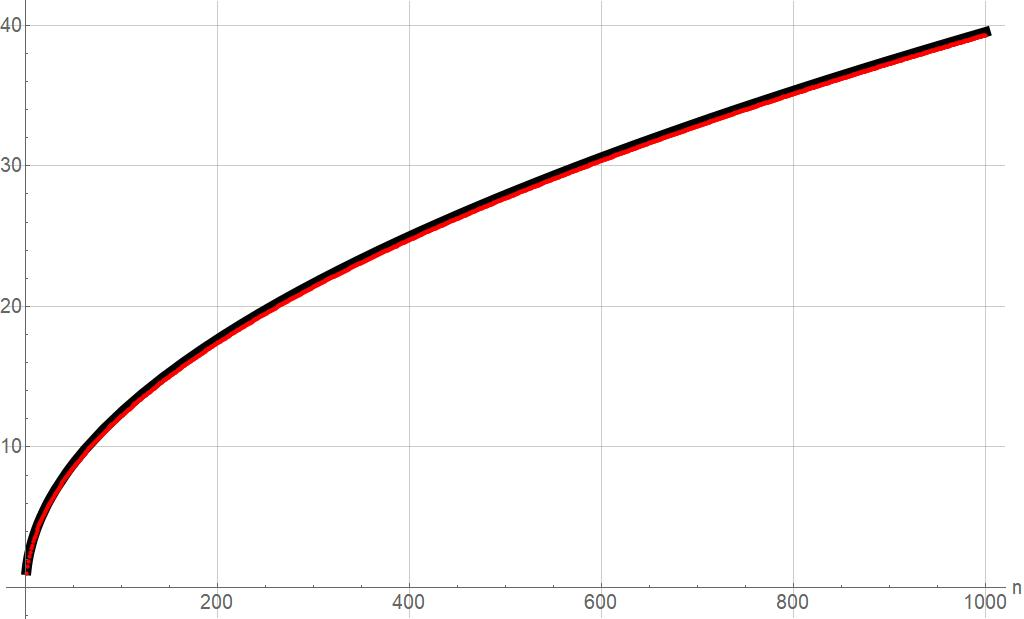
\includegraphics[width=0.75\textwidth]{Comp2.jpg}
	\caption{График зависимости среднего максимального числа компонент графа отображения от мощности языка}
	\label{Comp2}
\end{figure}

Если вынести из под знака суммы $\sqrt{n}$, то можно заметить, что функция стремится к некоторой константе не превосходящей $1.25$ (вывод делался при мощностях алфавита меньших 1000), подсчитав сумму при $n=10 000$, мы получим число $n=1.2499$.Отсюда следует что данная сумма должна сходиться к данной константе. График \ref{Comp2} показывает это.

\begin{theorem}
Таким образом функция, которая асимптотически приближается к данным числам, имеет вид
$$
\frac 5 4\sqrt{x}
$$
\end{theorem}

\subsection{Анализ третьего раздела}

Как всегда начнем с вывода явной формулы чисел

$$
\frac{F_b(z,x)}{1-x} =
(\gcd(r,1)x + \gcd(r,2)\frac{x^2}{2} + ... + \gcd(r,r)\frac{x^r}{r} + \gcd(r,1)\frac{x^{r+1}}{r+1} + ...)(1+x+x^2+x^3+...)=
$$
Для простоты расчетов можно считать, что мы работаем с языком мощности кратной $r$

$$
\sum_{k=1}^{\infty} (\sum_{p=1}^r\gcd(r,p)\sum_{z=0}^{k/r-1}\frac{1}{z r+p})x^k
$$

Таким образом коэффициент при $x^k/k!$ будет

$$
n!\sum_{p=1}^r\gcd(r,p)\sum_{z=0}^{k/r-1}\frac{1}{z r+p}
$$

Формулу можно записать проще и при этом она будет работать при любых $k$

\begin{theorem}
	Суммарное число компонент графа образующихся в результате итерации всех биективных отображений алфавита мощности $n$ в себя
$$
k!\sum_{p=1}^k \frac{\gcd(r,p)}{p}
$$
\end{theorem}

Из этой формулы можно сразу дать грубую верхнюю оценку для числа компонент, и т.к. $\gcd(r,p)\le r$, то имеет место теорема
\begin{theorem}
	 полученное число не превосходит значения функции:
$$
r(\log(n)+\gamma)
$$
, при достаточно больших $n$ и $r\ge 2$
\end{theorem}


\chapter*{Вывод}
\addcontentsline{toc}{chapter}{Вывод}

В данной курсовой работе были получены основные формулы, которые помогут читателю в дальнейшем в создании более совершенных алгоритмов шифрования и выработки ключа. 

В дальнейшем данная работа будет развиваться, можно получить более совершенные формулы аппроксимирования выведенных в 1 и 3 разделе второй главы числовых последовательностей, а также будет дано более математически корректное обоснование того, что последовательность из второго раздела второй главы асимптотически сходится к функции $5/4\sqrt{x}$.  

\addcontentsline{toc}{chapter}{Литература}
\bibliographystyle{utf8gost705u}
\bibliography{biblio}


\end{document}